\documentclass[10pt, a4paper]{article}

%%%%%%%%%%%%%%
%  Packages  %
%%%%%%%%%%%%%%


\usepackage{page_format}
\usepackage{special}
\usepackage{hyperref}
\usepackage{tikz}
\usepackage[compat=1.1.0]{tikz-feynman}
\usepackage[font=small,labelfont=bf,
   justification=justified,
   format=plain]{caption}
%----------------------------------------------------------------------
%\usepackage{amssymb} % Mathematical fonts.
%\usepackage{amsfonts} % Mathematical fonts.
\usepackage[nice]{nicefrac} % Nicer fractions
\usepackage{braket} % Dirac Notation.
\usepackage{bbm} % More bold fonts.
%\usepackage{mathrsfs} % Mathematical fonts.
\usepackage{esint} % Integrals
\usepackage{cancel} % Allows to scratch expressions.
\usepackage{mathtools} % Tools for math formating.
\usepackage{slashed} % Allows to slash individual characters.
\usepackage{xargs} % Better handling of optional arguments for commands
%----------------------------------------------------------------------
%\usepackage{lmodern} % Fonts.
\usepackage{feyn} % Feynman Diagrams in mathmode

%%%%%%%%%%%%%%%%%%%%%%%%%%%
% Mathématiques et physique
%%%%%%%%%%%%%%%%%%%%%%%%%%%%
% SI Units -----------------------
% The package 'siunitx' causes unresolved crashes (as of 22/08/31)
\newcommand{\ampere}{\text{A}}
\newcommand{\bell}{\text{B}}
\newcommand{\celsius}{\degree\text{C}}
\newcommand{\coulomb}{\text{C}}
\newcommand{\degree}{\,^{\circ}}
\newcommand{\farad}{\text{F}}
\newcommand{\electro}{\text{e}}
\newcommand{\gram}{\text{g}}
\newcommand{\henry}{\text{H}}
\newcommand{\hertz}{\text{Hz}}
\newcommand{\hour}{\text{h}}
\newcommand{\joule}{\text{J}}
\newcommand{\kelvin}{\text{K}}
\newcommand{\meter}{\text{m}}
\newcommand{\minute}{\text{m}}
\newcommand{\mole}{\text{mol}}
\newcommand{\newton}{\text{N}}
\newcommand{\ohm}{\Omega}
\newcommand{\pascal}{\text{Pa}}
\newcommand{\rad}{\text{rad}}
\newcommand{\second}{\text{s}}
\newcommand{\tesla}{\text{T}}
\newcommand{\torr}{\text{Torr}}
\newcommand{\volt}{\text{V}}
\newcommand{\watt}{\text{W}}
%
\newcommand{\tera}{\text{T}}
\newcommand{\giga}{\text{G}}
\newcommand{\mega}{~\text{M}}
\newcommand{\kilo}{~\text{k}}
\newcommand{\deci}{\text{d}}
\newcommand{\centi}{\text{c}}
\newcommand{\milli}{\text{m}}
\newcommand{\micro}{\mu}
\newcommand{\nano}{\text{n}}
\newcommand{\pico}{\text{p}}
\newcommand{\femto}{\text{f}}
%
\newcommand{\units}[1]{\text{#1}}
\newcommand{\tothe}[1]{\textsuperscript{#1}}
%
\newcommand{\per}{\text{/}}
%
\newcommand{\Time}[3]{#1\hour~#2\minute~#3\second} % TODO Optional arguments.
\newcommand{\Angle}[3]{#1^{\circ}~#2'~#3''} % TODO Optional arguments.


% Better epsilon -----------------------
\let\oldepsilon\epsilon
\let\epsilon\varepsilon
\let\varepsilon\oldepsilon


% Better \bar -----------------------
\renewcommand{\bar}[1]{\mkern 1.5mu\overline{\mkern-1.5mu#1\mkern-1.5mu}\mkern 1.5mu}


% Équations -----------------------
\newcommand{\al}[1]{\begin{align} #1 \end{align}} % Numbered equation(s),
\newcommand{\eqn}[1]{\begin{align*} #1 \end{align*}} % Number-less equation(s),
\newcommand{\sys}[1]{\begin{dcases*} #1 \end{dcases*}} % System of equations.


% Exponents -----------------------
\newcommand{\Exp}[1]{\text{e}^{#1}}		% e^#
\newcommand{\E}[1]{\times 10^{#1}}		% X 10^#


% Delimiters -----------------------
\newcommand{\p}[1]{\left( #1 \right)}	% (#)
\newcommand{\cro}[1]{\left[ #1 \right]}	% [#]
\newcommand{\abs}[1]{\left| #1\right|}	% |#|
\newcommand{\avg}[1]{\left\langle #1 \right\rangle} % <#>
\newcommand{\acc}[1]{\left\lbrace #1 \right\rbrace} % {#}


% Vectors -----------------------
\newcommand{\ve}[1]{\mathbf{#1}} % Upright bold face.
\newcommand{\vu}[1]{\hat{\ve{#1}}} % Hat vector upright bold face
\newcommand{\tens}{\otimes} % Tensor product
\newcommand{\nablav}{\bm{\nabla}} % Bold gradient


% Trig. functions with automatic formating  -----------------------
\newcommandx{\Sin}[2][1={}]{\text{sin}^{#1}\!\p{#2}}
\newcommandx{\Cos}[2][1={}]{\text{cos}^{#1}\!\p{#2}}
\newcommandx{\Tan}[2][1={}]{\text{tan}^{#1}\!\p{#2}}
\newcommandx{\Csc}[2][1={}]{\text{csc}^{#1}\!\p{#2}}
\newcommandx{\Sec}[2][1={}]{\text{sec}^{#1}\!\p{#2}}
\newcommandx{\Cot}[2][1={}]{\text{cot}^{#1}\!\p{#2}}
\newcommandx{\Arcsin}[2][1={}]{\text{arcsin}^{#1}\!\p{#2}}
\newcommandx{\Arccos}[2][1={}]{\text{arccos}^{#1}\!\p{#2}}
\newcommandx{\Arctan}[2][1={}]{\text{arctan}^{#1}\!\p{#2}}
\newcommandx{\Sinh}[2][1={}]{\text{sinh}^{#1}\!\p{#2}}
\newcommandx{\Cosh}[2][1={}]{\text{cosh}^{#1}\!\p{#2}}
\newcommandx{\Tanh}[2][1={}]{\text{tanh}^{#1}\!\p{#2}}


% Matrices -----------------------
\newcommand{\mat}[1]{\begin{bmatrix} #1 \end{bmatrix}} % Matrices with hooks.
\newcommand{\pmat}[1]{\begin{pmatrix} #1 \end{pmatrix}} % Matrices with parentheses.
\newcommand{\deter}[1]{\abs{\begin{matrix} #1 \end{matrix}}} % Determinant.
\newcommandx{\mO}[2][1={}, 2={}]{ \def\temp{#2}\ifx\temp\empty\ve{O}_{#1}\else\ve{O}_{#1\times #2}\fi}% Zero matrix.
\newcommandx{\mI}[2][1={}, 2={}]{ \def\temp{#2}\ifx\temp\empty\ve{I}_{#1}\else\ve{O}_{#1\times #2}\fi}%  Identity matrix.
\newcommand{\Det}[1]{\text{det}\p{#1}} % det(#)
\newcommand{\Tr}[1]{\text{Tr}\p{#1}} % Tr(#)


% Derivatives -----------------------
\newcommand{\D}{\text{d}} % Differential 'd'.
\newcommandx{\dd}[3][1={},3={}]{\frac{\D^{#3}#1}{\D{#2}^{#3}}} % Total derivative according to #2, #1 is the function and #3 is the order.
\newcommand{\del}{\partial} % Partial 'd'.
\newcommandx{\ddp}[3][1={},3={}]{\frac{\del^{#3}#1}{\del{#2}^{#3}}} % Dérivée partielle selon #2, #1 est la fonction est #3 est l'ordre.
\newcommand{\eval}[1]{\left. {#1} \right|} % Bar on the right of expression.
\newcommand{\delbar}{\slashed{\del}} % Partial Inexact differential.
\newcommand{\dbar}{\dj}% Inexact differential.


% Integrals -----------------------
\newcommand{\intinf}{\int\displaylimits_{-\infty}^{\infty}} % From -00 to 00.
\newcommandx{\Int}[2][1={},2={}]{\int\displaylimits_{#1}^{#2}} % Faster bounded integrals.


% Complex numbers -----------------------
\renewcommand{\Re}[1]{\text{Re}\acc{#1}} % Re{#}
\renewcommand{\Im}[1]{\text{Im}\acc{#1}} % Im{#}


% Sets -----------------------
\newcommand{\N}{\mathbbm{N}} % Natural numbers.
\newcommand{\Z}{\mathbbm{Z}} % Integers.
\newcommand{\Q}{\mathbbm{Q}} % Rational numbers.
\newcommandx{\R}[1][1={}]{\mathbbm{R}^{#1}} % Real numbers.
\newcommandx{\C}[1][1={}]{\mathbbm{C}^{#1}} % Complex numbers.
\newcommandx{\F}[1][1={}]{\mathbbm{F}^{#1}} % Some field.
\newcommand{\M}[3]{\mathbb{M}_{#1\times#2}(#3)}	% Matrices.
\newcommand{\Po}[2]{\mathbb{P}_{#1}(#2)} % Polynomials.
\newcommand{\Lin}{\mathbb{L}} % Linear maps.


% Constants and physical symbols -----------------------
\newcommand{\eo}{\epsilon_0} % epsilon 0.
\renewcommand{\L}{\mathcal{L}} % Lagrangian.

\usepackage{listings,xcolor}

% Default fixed font does not support bold face
\DeclareFixedFont{\ttb}{T1}{txtt}{bx}{n}{12} % for bold
\DeclareFixedFont{\ttm}{T1}{txtt}{m}{n}{12}  % for normal

\lstset{language=Mathematica}
\lstset{basicstyle={\sffamily\footnotesize},
  numbers=left,
  numberstyle=\tiny\color{gray},
  numbersep=5pt,
  breaklines=true,
  captionpos={t},
  frame={lines},
  rulecolor=\color{black},
  framerule=0.5pt,
  columns=flexible,
  tabsize=2
}

\usepackage{color}
\definecolor{deepblue}{rgb}{0,0,0.5}
\definecolor{deepred}{rgb}{0.6,0,0}
\definecolor{deepgreen}{rgb}{0,0.5,0}

\newcommand\pythonstyle{\lstset{
language=Python,
basicstyle=\footnotesize,
morekeywords={self},              % Add keywords here
keywordstyle=\color{deepblue},
emph={MyClass,__init__},          % Custom highlighting
emphstyle=\color{deepred},    % Custom highlighting style
stringstyle=\color{deepgreen},
frame=tb,                         % Any extra options here
showstringspaces=false
}}

\lstnewenvironment{python}[1][]
{
\pythonstyle
\lstset{#1}
}
{}

% References
\usepackage{biblatex}
\addbibresource{ref.bib}


%%%%%%%%%%%%
%  Colors  %
%%%%%%%%%%%%
% ! EDIT HERE !
\colorlet{chaptercolor}{red!70!black} % Foreground color.
\colorlet{chaptercolorback}{red!10!white} % Background color


%%%%%%%%%%%%%%
% Page titre %
%%%%%%%%%%%%%%
\title{Homework 1} % Title of the assignement.
\author{\PA} % Your name(s).
\teacher{Emilie Huffman and Giuseppe Sellaroli} % Your teacher's name.
\class{Statistical Physics} % The class title.

\university{Perimeter Institute for Theoretical Physics} % University
\faculty{Perimeter Scholars International} % Faculty
%\departement{<Departement>} % Departement
\date{\today} % Date.


%%%%%%%%%%%%%%%%%%%%%%
% Begin the document %
%%%%%%%%%%%%%%%%%%%%%%
\begin{document}

% Make the title page.
\maketitlepage

% Make table of contents
\maketableofcontents

% Assignment starts here ----------------------------

\footnotesize{
\section{Critical exponent for the coexistence boundary}
\begin{enumerate}
  \item[(a)] Consider a thermodynamical system described by the Helmotz free energy $F$ depending on temperature $T$, volume $V$ and particle number $N$. Pressure is related to $T, V$ at fixed $N$ with $P= -\left.\frac{\partial F}{\partial V}\right|_{T, N} = f(T, V)$ where the function $f$ forms a state equation. We assume the state equation is consistent with a second-order phase transition at $T_c, V_c, P_c$ (highest pressure inflection point of $P, V$ isotherms). Furthermore, in a $P, V$ diagram, this point is taken to join the first-order phase transition lines of liquid-coexistence and coexistence-gas transitions. These lines respectively mark the end of a lower volume liquid phase and higher volume gas phase at pressures $P<P_c$. For $P> P_c$ there is no distinction between the liquid and gas phases. In what follows, volume dependence is replaced by reduced volume $v = V/V_c$ and we also use reduced temperature $t=T/T_c$. We are interested in the behavior of the liquid-coexistence transition volume $v_l$ and gas-coexistence transition volume $v_g$ on $t \sim 1$ isotherms. We can express $v_l$ and $v_g$ with their respective deviation from $v = 1$ as $v_l = 1 - x$ and $v_g = 1 + y$ with $x , y \ge 0$ (only moving to sides of the coexistence region where pressure is smooth). Supposing $x, y$ are small, we perform a reduced volume Taylor expansion of the pressure on an isotherm with temperature $T \sim T_c$ to write 
  \begin{align*}
    P(T, v) =  P(T, 1) + a(T) (v-1) + b(T) (v-1)^2 + c(T) (v-1)^3 + O((v-1)^4)
  \end{align*}
  where $a(T), b(T) \neq 0$. The defining characteristic of the transition lines is that their points at a given temperature have the same pressure and chemical potential $\mu$. Expressing the chemical potential with the Gibbs free energy $G = \mu N$, we have 
  \begin{align*}
    P(T, v_l) = P(T, v_g) \quad \& \quad  \left.\frac{G}{N}\right|_{T, v=v_l, N} = \left.\frac{G}{N}\right|_{T, v=v_g, N}
  \end{align*}
  where the pressure dependence of the Gibbs free energy is formally replaced with volume dependence using the state equation. Using the above Taylor expansion truncated from $O((v-1)^4)$, the pressure constraint reads 
  \begin{align*}
    P(T, v_l) &= P(T, 1) + a(T) (1-x - 1) + b(T) (1-x-1)^2 + c(T) (1-x-1)^3\\
    &= P(T, 1) + a(T) (1+y-1) + b(T) (1+y-1)^2 + c(T) (1+y-1)^3 = P(T, v_g)\\
    &\iff 0 = a(T) (x + y) + b(T) (y^2 - x^2) + c(T) (y^3 + x^3). \tag{$\star$} \label{1}
  \end{align*}
  To relate chemical potential $\mu$ to pressure and volume, we use the fact temperature should not vary on the isotherms. At fixed $N$ and $T$, the free energy differencial reduces to $dG = V dP$. To ensure that the chemical potentials are the same at $v_l$ and $v_g$, there has to be no change in $G/N$ between those volumes. Integrating the change on an isotherm (the change in a thermodynamic potential between two points is path independent) yields 
  \begin{align*}
    0 &= \left.\frac{G}{V_c N}\right|_{T, v=v_l, N} - \left.\frac{G}{V_c N}\right|_{T, v=v_g, N} = \dfrac{1}{N} \int_{P(T, v_l)}^{P(T, v_g)} v \ dP\\
    &= \dfrac{1}{N} \int_{v_l}^{v_g} v \left.\frac{\partial P}{\partial v}\right|_{T, N} dv = \dfrac{1}{N} [P(T, v)v]_{v_l}^{v_g} - \dfrac{1}{N} \int_{v_l}^{v_g} P(T, v) \ dv \\
    &= \dfrac{1}{N} \left[P(T, v)v - P(T, 1)v - \frac{1}{2} a(T) (v-1)^2 - \frac{1}{3} b(T) (v-1)^3 + O((v-1)^4)\right]_{v_l}^{v_g}\\ 
    \iff 0 &= (P(T, 1)-P(T, 1))(v_g-v_l) + a(T) (x + y) + b(T) (y^2 - x^2) + c(T) (y^3 + x^3)\\
    &\quad- (a(T) (-x) + b(T) (-x)^2 + c(T) (-x)^3) (-x) + (a(T) y + b(T) y^2 + c(T) y^3) (+y) - \frac{1}{2} a(T) (y^2 - x^2) - \frac{1}{3} b(T) (y^3 + x^3)\\
    &= a(T) (x + y) + \left(b(T) + \frac{1}{2}a(T)\right) (y^2 - x^2) + \left(c(T) + \frac{2}{3}b(T)\right) (y^3 + x^3) \tag{$\star \star$} \label{2}
  \end{align*}
  where the integral was evaluated using the Taylor expansion of $P$.  
  
  \item[(b)] Substracting \eqref{1} from \eqref{2}, we get 
  \begin{align*}
    0 = \frac{1}{2}a(T) (y^2 - x^2) + \frac{2}{3}b(T) (y^3 + x^3) \iff 0 = 3a(T) (y^2 - x^2) + 4 b(T) (y^3 + x^3).  \tag{$\star\star\star$} \label{3}
  \end{align*}
  We can now assume the deviation $x, y$ for a fixed pressure can be related by a temperature-dependent Taylor expansion of $y$ in terms of $x$. To preserve the validity of our previous truncations, we need to have $y \propto x$ ($x$ and $y$ are close deviations) so that all the terms pushed beyond $O(x^3)$ stay truncated. A constant term in the expansion of $y$ would shift terms from higher orders to our truncated expansion and \eqref{3} would not hold. We can also conclude $y \propto x$ from the fact $x=0 \implies y=0$ since the two transition lines are joined at the critical point. Substituting $y = d(T) x + e(T) x^2 + f(T) x^3 + O(x^4)$ in a second order expansion in $x$ of \eqref{3} yields 
  \begin{align*}
    0 = 3a(T) (d(T)^2 x^2 - x^2) \iff d(T) = \pm 1. 
  \end{align*}
  Since $x$ is positive, we can find a neighborhood of $v=1$ where the linear term in the expansion of $y$ dominates and imposes $d(T) = 1$. We finally have $y = x + O(x^2)$ which translates to $|v_g-1| \sim |v_l-1|$ for $t \to 0^-$.

  Note: This result appears to be inconsistent with \eqref{1} and \eqref{2} because substituting $y =  + O(x^2)$ leads the first order term to be $a(T)(x + y) = 0$ which is impossible since $x, y > 0$ and $a(T) \neq 0$. As we get close to the critical point, the first derivative of pressure vanishes making the $b(T)$ term more significant in these cubic equations. This suggests a possible solution to the apparent problem (analogous to the perturbation theory used to solve polynomial equations by expanding in powers of a small coefficient): the ultimate expansion parameter is temperature deviation $t$. Expanding $x$ and $y$ in terms of this perameter will allow powers (possibly fractionnal) to mix with the power expansion of $a(T)\sim t, b(T)\sim 1$ near the critical temperature. Terms at first order in temperature coming from $x+y$ will be shifted to second order and mix with the zeroth order contribution of $b(T)$.
\end{enumerate}

\section{Dietrici equation of state}
\begin{enumerate}
  \item[(a)] To investigate the universality of critical exponents characterizing phase transitions, we consider the Dietrici equation of states 
  \begin{align*}
    P(v-b) = kT \exp\left(-\frac{a}{kT v}\right), \quad a, b > 0
  \end{align*} 
  describing a gas with pressure $P$ and volume $v$ per particle at temperature $T$. Figure \ref{f1} represents characteristic isotherms associated with this equation of states. 

  \begin{figure}[h!]
    \centering
    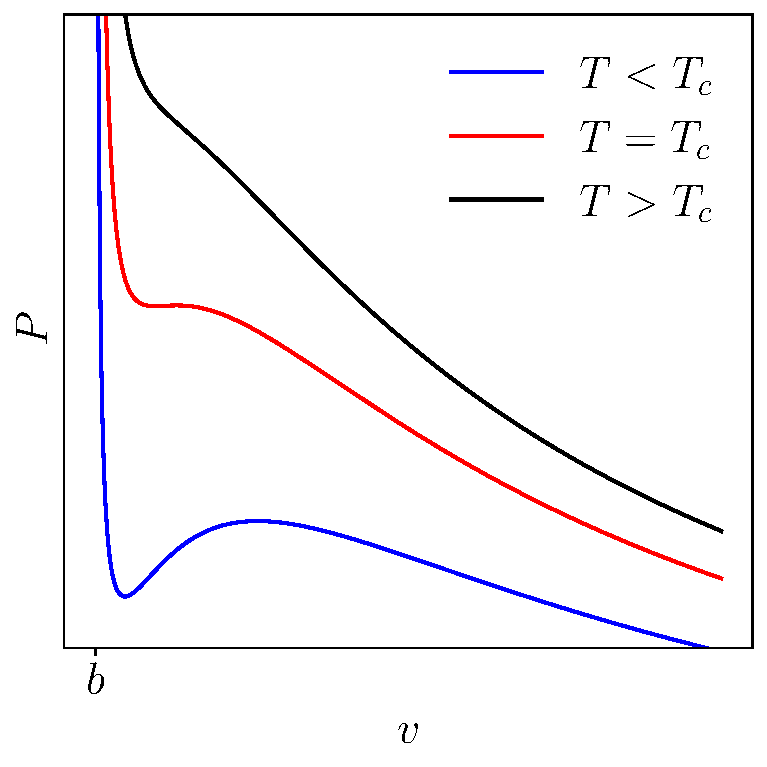
\includegraphics[scale=0.5]{C:/Users/pgraham1/Documents/GitHub/PSI/Statistical_Physics/Homework1/TeX-JAM/Isotherms.pdf}
    \caption{\label{f1} Sketch of the three types of isotherms found in the $P, v$ diagram of the Dietrici equation of states. For $T=T_c$ is the temperature at which a sign vanishing derivative point appears in the isotherms (it is also an inflection point). Higher temperatures have no such point and lower temperatures have two local extrema. Globally, these characteristics are analogous to the isotherm structure of the Van der Waals equation of states.}
  \end{figure}

  The critical temperature $T_c$ is the temperature at which an isotherm features an inflection point. At this point, the two extrema for $P(v)$ for isotherms with $T < T_c$ are brought together and the first derivative of  $P(v)$ has only one degenerate root. This implies that  
  \begin{align*}
    0 = \left.\frac{\partial P}{\partial v}\right|_{T_c, v_c} = \frac{- T_c k v_c^{2} - a \left(b - v_c\right)}{v_c^{2} \left(b - v_c\right)^{2}} e^{- \frac{a}{T_c k v_c}} \quad \text{with degenerate root} \implies a^2 - 4 T_c k a b = 0 \quad \text{discriminant}\implies T_c = \frac{a}{4k b}
  \end{align*}
  where the derivative was computed using the following sympy code 
  \begin{python}
import sympy as sp 

T, a, b, v, k = sp.symbols("T a b v k")

P = k * T * sp.exp(-a/(k * T * v))/(v-b)

del1P = sp.diff(P, v, 1).simplify()
  \end{python}
Solving for the critical volume $v_c$ yields 
\begin{align*}
  0 = -\frac{a}{4k b} k v_c^{2} - a \left(b - v_c\right) \iff 0 = v_c^{2} + 4 b^2 - 4 v_c b = (v_c - 2 b)^2 \iff v_c = 2b. 
\end{align*}
The associated critical pressure is obtained by substituting the expression for $v_c$ and $T_c$ in $P(v)$. We get 
\begin{align*}
  P_c = \dfrac{ka}{4k (2b-b)b} \exp\left(-\frac{4k ab}{2k ab}\right) = \dfrac{a}{4b^2} \exp\left(-2\right). 
\end{align*} 
To simplify further calculations we reexpress the equation of states with reduced pressure volume $v_r = v/v_c$, $P_r = P/P_c$ and $T_r = T/T_c$. 
\begin{align*}
  P_r = \frac{P}{P_c} = \frac{kT}{b(2v_r-1)} \exp\left(-\frac{2a}{4 b kT v_r}\right) \dfrac{4b^2}{a} \exp\left(+2\right) = \frac{T_r}{2v_r-1} \exp\left(2-\frac{2}{T_r v_r}\right).
\end{align*} 
\newpage
  \item[(b)] Around the critical volume $v_r = 1$ and we can do an of the expansion of the reduced volume $v_r = 1 + x$. The pressure associated to the deviation $x$ on the $T_r=1$ isotherm is given by 
  \begin{align*}
    P_r = \frac{T_r}{2(1+x)-1} \exp\left(2-\frac{2}{T_r (1+x)}\right) \approx 1 - \frac{2 x^{3}}{3} + O\left(x^{4}\right).  
  \end{align*}
  which is expected because, at the inflection point, the first and second derivatives vanish. The previous expansion was computed using the following sympy code 
  \begin{python}
import sympy as sp 

vr, x = sp.symbols("vr x")

P = sp.exp(2-2/vr)/(2*vr - 1)
P = P.subs({vr:1+x}).series(x, 0, 4)
  \end{python}
  Using the previous expansion, we can solve for $x$ as a function of $P_r$ leading to 
  \begin{align*}
    x = v_r-1 = -\frac{3}{2}\left(P_r - 1\right)^{1/3} \sim \left(P_r - 1\right)^{1/\delta}
  \end{align*}
  leading to the critical same critical exponent $\delta = 3$ as in the Van der Waals model. We this result to extract the $\gamma$ critical exponent describing the scaling of isothermal compressibility $k_T$ at $T_r = 1$ as a function of $P_r$. We have 
  \begin{align*}
    k_T = -\dfrac{1}{v_r}\left(\frac{\partial v_r}{\partial P_r}\right) \approx \frac{-\frac{3}{6}\left(P_r - 1\right)^{-2/3}}{-\frac{3}{2}\left(P_r - 1\right)^{1/3}} = -\frac{-\frac{3}{6}\left(P_r - 1\right)^{-2/3}}{-\frac{3}{2}\left(P_r - 1\right)^{1/3}} = -\frac{1}{3} \left(P_r - 1\right)^{-1} \sim (P_r - 1)^{-\gamma}
  \end{align*}
  which is consistent with $\gamma = 1$. 


  \item[(c)] Below the critical point, the temperature is expanded as $T_r = 1 - t$ with a small positive deviation $t$. At fixed pressure on the liquid-coexistence and coexistence-gas transition lines, the volumes are respectively $v_l$ and $v_g$. These volumes are expanded around $v_r = 1$ as $v_l = 1 - x$ and $v_g = 1 + y$ with respective positive deviations $x$ and $y$ associated with a small temperature shift $t$. From the calculations of question 1, we know that $y = x + c x^2 + O(x^3)$ \footnote{The quadratic term weighted by $c$ is considered here because it appears in a third order expansion in $x$ of $P_r(v_g, T_r)$, but it doesn't affect the critical exponent we find} is required by equality of chemical potential, pressure and critical temperature deviation $t$. With this in mind, we can relate the shifts $x$ and $t$ with the pressure equality condition. It reads  
  \begin{align*}
    P_r(v_l, T_r) = P_r(v_g, T_r) \implies  P_r(1+x, 1+t) = P_r(1-x + cx^2 + O(x^3), 1+t)
    \iff 0 = - 4 c t x^{3} + 2 c t x^{2} + 8 t x^{3} + 4 t x - \frac{4 x^{3}}{3}
  \end{align*} 
where the expansion was done using the following python code
\begin{python}
import sympy as sp 

vr, Tr, x, y, t, c = sp.symbols("vr Tr x y t c")

P = sp.exp(2-2/(Tr * vr))/(2 * vr - 1) * Tr

P = P.subs({Tr:1-t}).series(t, 0, 2).removeO()

Pl = P.subs({vr:1-x}).series(x, 0, 4) 
Pg = P.subs({vr:1+y}).series(y, 0, 4) 
Pg = Pg.subs({y : x + c * x ** 2})

Eq = (Pg-Pl).simplify().removeO()
\end{python}
This equation is solved for $x$ and expanded in $t$ again to get 
\begin{align*}
  x = \sqrt{3} \sqrt{t} + t^{\frac{3}{2}} \left(- \sqrt{3} \cdot \left(3 c - 6\right) + \frac{\sqrt{3} \cdot \left(\frac{3 c^{2}}{8} + 6 c - 12\right)}{4}\right) + \frac{3 c t}{4} + O\left(t^{2}\right) \sim t^{1/2} \sim t^{\beta}
\end{align*}
leading to $\beta = 1/2$. This step was completed with the code 
\begin{python}
  X = sp.solve(Eq, x)[1].series(t, 0, 2)
\end{python}
\end{enumerate}






\section{Acknowledgement}
Thanks to Thiago (neighborhood argument for the positivity of $d(T)$ in question 1), Yale, and Ruhi for discussions about the expansion of $y$ in terms of $x$ in question $1$ part (b). Thanks to  
}

% References
\makereferences
%-------------------------------------------------------


%%%%%%%%%%%%%%%%%%%%%%%%
% Terminer le document %
%%%%%%%%%%%%%%%%%%%%%%%%
\end{document}